\documentclass[brudnopis]{xmgr}
% Jeśli nowe rozdziały mają się zaczynać na stronach
% nieparzystych:
%\documentclass[openright]{xmgr}

%\defaultfontfeatures{Scale=MatchLowercase}
%\setmainfont[Numbers=OldStyle,Ligatures=TeX]{Minion Pro}
%\setsansfont[Numbers=OldStyle,Ligatures=TeX]{Myriad Pro}
% for fontspec version < 2.0
\setmainfont[Numbers=OldStyle,Mapping=tex-text]{Minion Pro}
\setsansfont[Numbers=OldStyle,Mapping=tex-text]{Myriad Pro}
%\setmonofont[Scale=0.75]{Monaco}

% Opcjonalnie identyfikator dokumentu
% drukowany tylko z włączoną opcją 'brudnopis':
\wersja   {wersja wstępna [\ymdtoday]}

\author   {Czerwińska Agnieszka}
\nralbumu {206\,314}
\email    {czewinska.agnieszka.lucja@gmail.com}

\author   {Maciejewski Michał}
\nralbumu {206\,316}
\email    {michal.maciejewski92@gmail.coml}

\author   {Miszczykowski Mariusz}
\nralbumu {000\,000}
\email {000@gmail.com}

\title    {Tworzenie gier na przykładzie silników Unity i Unreal Engine}
\date     {2016}
\miejsce  {Gdańsk}

\opiekun  {dr W. Bzyl}

% dodatkowe polecenia
%\renewcommand{\filename}[1]{\texttt{#1}}
%\definecolor{stress}{cmyk}{0,1,0.13,0} % RubineRed
%\definecolor{topic}{cmyk}{0.98,0.13,0,0.43} % MidnightBlue
\usepackage{listings}

\begin{document}

% streszczenie
\begin{abstract}
  W pracy opisano współczesne podejście do programowania gier z wykorzystaniem silników gier.
  Porównano dwa silniki o otwartym kodzie: Unreal Engine udostępnianym przez firmę Epic Games, oraz Unity 3D –- Unity Technologies. 

 W części praktycznej pracy stworzono dwie wersje gry „The Climb” - po jednej w każdym z silników. Zostały one oparte na jednym Game Design Document (patrz, rozdział 3 –- „Czym jest Game Design Document”).

 Pozwoliło to na stworzenie gier o podobnych cechach, jednak dzięki specyfice samego dokumentu, także nie ograniczających możliwości żadnego z silników. Cały przebieg procesu tworzenia owych gier został opisany w oddzielnych rozdziałach.
\end{abstract}

% słowa kluczowe
\keywords{gry konsolowe, 
silnik gier, 
Unity, 
Unreal Engine, 
animacja,
fizyka,
skrypty,
interfejs użytkownika,
scena,
obiekt,
platforma,
optymalizacja,
particle,
audio,
3D,
architektura,
oswietlenie,
komponent,
drag and drop}

% tytuł i spis treści
\maketitle

% wstęp
\introduction

Jeszcze 20 lat temu tworzenie gier było nie lada wyzwaniem, wymagało ogromnej cierpliwości, sporej wiedzy z zakresu fizyki, informatyki i matematyki. Dzisiaj zaawansowane oprogramowanie do tworzenia gier znacząco ułatwia tworzenie tego typu rozrywki. Dlatego liczba gier wychodzących na rynek jest tak duża, że nie sposób śledzić pomniejsze tytuły.

Gry komputerowe towarzyszyły nam od dzieciństwa. Były naszym hobby i poświęcaliśmy im mnóstwo czasu. Od zawsze marzyliśmy, by zacząć tworzyć swoje własne gry. 
Wiedza, którą zdobyliśmy w trakcie studiów pozwoliło nam nie tylko na realizację tego marzenia, ale dała nam również możliwość analizy różnych sposobów tworzenia oprogramowania. W tej pracy chcemy przedstawić różnice wynikające z oparcia jednej gry na dwóch silnikach do tworzenia gier - Unity i Unreal Engine. W tej pracy zawarliśmy podstawowe różnice między nimi, ich głowne zalety, jak i ograniczenia obu silników. Wierzymy, że pozwoli to początkującym twórcom gier, jak i tym bardziej doświadczonym, znaleźć właściwe narzędzie do wykonania zadania.

Silniki gier to zaawansowane oprogramowanie tworzone przez firmy, specjalnie na potrzeby nowych gier. Powołanie nowej gry do życia wymaga ogromnych nakładów czasowych i finansowych. „Jak będziemy generować grafikę? Czy w naszej grze będzie realistyczna fizyka? A dynamiczne światło? Co z dzwiękiem? Jaki język programowania wybrać? A i trzeba jeszcze tę grę zoptymalizować pod konkretną platformę!" Na te i wiele innych pytań trzeba odpowiedzieć za każdym razem tworząc nową grę. Doświadczeni twórcy wiedzą jednak, że to własnie odpowiedzi na te pytania generują największe koszty. Aby uniknąć odkrywania koła na nowo, firmy często tworzą własne silniki, bądź wykupują licencje na inne. Współcześnie, większość nowych tytułów robiona jest na już gotowych silnikach. Tylko mały procent doczeka się własnego, wartego niejednokrotnie więcej niż sama gra. 
Na nasze szczęście dzisiaj każdy z nas może skorzystać z możliwości takiego silnika. 

Mimo, że na rynku istnieje wiele innych darmowych silnikow, w tej pracy skupimy sie na dwóch obecnie najpopularniejszych darmowych silnikach:
Unreal Engine udostępniane przez firmę Epic Games, oraz Unity 3D udostępniane przez firmę Unity Technologies. 

Przyjrzymy się krótkiej historii silników gier oraz porównamy oba oprogramowania. Dowiemy sie czym jest GDD, następnie przyjrzymy się ich cechom i opiszemy proces tworzenia gier w każdym z nich. Odkryjemy najczęstsze bugi w grach i jak z nimi walczyć, a w podsumowaniu opiszemy krótko: stopień trudnosci w użytkowaniu, czas potrzebny do stworzenia gry i zastanowimy sie nad przyszłością obu silników.

\chapter{Krótka historia silników do tworzenia gier}

Silnik gier jest to specjalne oprogramowanie zaprojektowane z myślą o tworzeniu i rozbudowywaniu gier wideo. Jego typową funkcjonalnością jest obsługa generowania grafiki (zarówno 2D i 3D), fizyki, kolizji, dźwięku, sieci, animacji, procesora, pamięci itp. Większość silników opiera się na tzw. skryptach – krótkich programach pisanych wewnątrz aplikacji, pozwalających na stosunkowo nieskrępowaną modyfikację i ciągłe rozszerzanie możliwości danego silnika. Idzie to w parze z głównym założeniem jakim jest możliwość jego wielokrotnego wykorzystania do tworzenia kompletnie odmiennych tytułów.  

Teoretycznie prawie każda gra, która kiedykolwiek powstała, opiera się na jakimś silniku. Jednak dopiero lata 90' uznajemy za początek ich historii. Jest to związane z faktem, że pierwsze gry były tzw. „hardkodowane”. Oznacza to, że wszelkie dane były bezpośrednio wpisywane w kod źródłowy, a ich wartości dostosowane bezpośrednio do urządzenia na które były tworzone. Ze względu na niską wydajność i limity pamięci ówczesnych maszyn było to rozwiązanie konieczne. Uniemożliwiały jednak modyfikację kodu. Oznaczało to, że silnik wykorzystywany był tylko raz, pod konkretną grę, co stoi w konflikcie z wcześniej podaną definicją silnika gier.

Poniżej została zamieszczona tabelka z datami, autorami i szczególnymi cechami silników gier, poczynając od „Hovertank 3D”. Nie był to pierwszy silnik w historii, jednak jako pierwszy był rozwijany i użyty w wielu produkcjach. Był to także jeden z tytułów 3D z gatunku FPS ( ang. first-person-shooter ). Rozwój tego gatunku szedł w parze z powstaniem terminu „silnika gier”. Trzeba zaznaczyć, że ze względu na ogromną ilość różnych silników, poniższa lista nie jest kompletna i zawiera tylko te najpopularniejsze i/lub najbardziej zasłużone.

\begin{table}[!tbh]
\begin{tabular}{|p{2cm}|p{1,5cm}|p{2,7cm}|p{8cm}|} \hline
Nazwa & Rok powstania & Autor/właściciel & Szczegóły \\ \hline
Hovertank 3D & 1991 & John Carmack (id Software) & Silnik powstał w 6 tygodni, wielokrotnie rozwijany, napisany w językach C i x86 Assembly \\ \hline
Wolfenstein 3D & 1992 & John Carmack (id Software) & Usprawniona wersja Hovertank 3D, dodano raycasty, i fizykę gracza, zwiększono wydajność \\ \hline
ID Tech 1 & 1993 & John Carmack (id Software) & Pierwszy z serii silników id Tech, dodano opcje konfiguracji grafiki, otwarte przestrzenie, pełne oteksturowanie gry \\ \hline
Build & 1996 & Ken Silverman (3D Realms) & Dodano woksele, podział na sektory, destrukcja otoczenia \\ \hline
Quake Engine & 1996 & John Carmack (id Software) & Dodano statyczne oświetlenie, zwiększono wydajność, możliwość gry sieciowej, lightmapy \\ \hline
Unreal Engine & 1998 & Epic Games & Używany i rozwijany do dziś silnik gier, korzysta z własnego języka skryptowego UnrealScript, modularna budowa silnika, łatwy do modowania, napisany w C++, jeden z najpopularniejszych silników w historii \\ \hline
Id Tech 3 & 1999 & id Software & Powstał w odpowiedz na UnrealEngine, wymaga Open GL, dodanie shaderów,  dodano format MD3 do modeli 3D \\ \hline
Infernal Engine & 2000 & Terminal Reality & Napisany w C++, język skryptowy Dante, niewymagający kompilacji przy zmianach, rozbudowany system zarządzania zasobami \\ \hline
Cry Engine & 2004 & Crytek & Powstało wstępnie jako demo technologiczne karty graficznej GeForce 3, obsługa Shader Model 3.0, efekt HDR,  język programowania Lua i C\# \\ \hline
Source Engine & 2004 & Valve Corporation & Napisany w C++, Source SDK udostępniany dla każdego użytkownika posiadającego grę na platformie Steam, wsparcie wieloprocesowości \\ \hline
Unity Engine & 2005 & Unity Technologies & Napisany w C, C++ i C\#, pozwala robić gry na większość istniejących platform, łatwy w użytkowaniu \\ \hline
Frostbite & 2008 & Digital Illusions CE & HDR Audio, system destrukcji otoczenia \\ \hline

\end{tabular}
\caption{Skrócona historia silników gier
  typu dokumentu\label{tab:dtd-cmp}}
\source{Wikipedia}
\end{table}

\chapter{Czym jest Game Design Document?}

Game Design Document (w skrócie GDD) jest dokumentem tworzonym jeszcze przed przystąpieniem do tworzenia gry. Najważniejszym celem dokumentu jest utrzymanie spójności oraz jednoznaczne wytyczenie celów związanych z projektem. GDD jest tak zwanym „żywym” dokumentem. Oznacza to, że może on być rozwijany i zmieniany podczas pracy nad grą. Jeśli pojawią się przeszkody uniemożliwiające wykonanie wcześniejszych założeń, lub powodujące znaczne opóźnienie w pracach nad grą dozwolone jest zmienianie danych części dokumentu. Zaleca się jednak w miarę możliwości, aby nie odchodzić za daleko od wyjściowych założeń, gdyż stoi to w konflikcie z założeniami owego dokumentu. 

Struktura dokumentu nie jest jednoznacznie zdefiniowana. W zależności od wielkości zespołu oraz docelowych odbiorców może on przybierać różnorakie formy – od czysto formalnych mocno technicznych aspektów, do ogólnej wizji artystycznej świata i rodzaju rozgrywki. Dokument może składać się z czystego tekstu, ale również screenów, zdjęć, szkiców koncepcyjnych, diagramów. Każda forma jak najlepiej oddająca założenia gry jest akceptowalna. 

Zdarza się, że GDD często zaczyna się tylko podstawowymi założeniami gry, a kończy jako rozbudowany wielostronicowy dokument opisujący każdy możliwy aspekt gry. Przy jego pisaniu nie można zapomnieć, że   będzie on czytany przez każdego członka zespołu tworzącego grę, nie tylko przez programistów, ale także artystów czy managerów. Dlatego pomimo ogólnej swobody przy jego pisaniu zaleca się zachowywać ogólnie pojętą strukturę, co pozwala na oddzielenie zagadnień typowo technicznych, od tych związanych z marketingiem czy kreacją świata. 

Wiele firm wymaga od twórców gier aby dostarczali GDD. Jako, że nie ma określonego standardu dla tego typu dokumentu, autorzy muszą go tak zaprojektować, aby grę nie tylko przedstawić, ale także „sprzedać”. Sprawia to, że GDD potrafią się od siebie znacząco różnić. 

Swoboda w tworzenia GDD daje wiele możliwości, ale potrafi także być sporym wyzwaniem. Osoby posiadające już doświadczenie przy robieniu gier zdecydowanie lepiej radzą sobie przy pisaniu takiego dokumentu, gdyż znają już wszystkie etapy produkcji, oraz problemy z nią związane. Korzystając z ich doświadczenia można nakreślić pewne prawidłowości przy jego pisaniu.

\section{Jak napisać dobre GDD}

Jeśli GDD pisze kilka osób, wyznacz jedną osobę odpowiedzialną za funkcjonowanie dokumentu. 
Zbyt duża swoboda  w dostępie do dokumentu wprowadza niepotrzebny chaos. Każdy pomysł przed wpisaniem powinien zostać najpierw rozpatrzony, aby nie wpuszczać do projektu nadmiarowych pomysłów.

Nie pisz całego dokumentu na „raz”.
Pamiętaj, że GDD tak samo jak projekt będzie ciągle ewoluować. Może się okazać, że wraz z rozwojem projektu, wiele pomysłów zostanie odrzuconych, a niektóre założenia ulegną zmianie. Jeśli nie pozostanie wystarczająco miejsca na zmiany, lub projekt zacznie przechodzić znaczące zmiany, może to zaważyć na czytelności dokumentu.

Używaj różnych form przekazu.
Obraz przy opisie lokacji, bądź referencja przy animacji powiedzą czytelnikowi więcej niż długi skomplikowany tekst. 

Podziel dokument na sekcje.
Stwórz dział „Użyte technologie” i „Świat gry”. W tym momencie każdy będzie wiedział, gdzie i jakiego typu informacje znajdują się w tekście.

Wyznacz realistyczne cele.
Zanim dokument zostanie ostatecznie zatwierdzony, powinien najpierw zostać rozpatrzony pod kątem potencjalnych kosztów czasowych i finansowych. Stworzenie wielkiego tytułu, może być zbyt ambitne dla małego zespołu. Głównym celem powinno być ukończenie gry w odpowiednim czasie. Trzeba wziąć pod uwagę ewentualne problemy i pamiętać, że każdy nowy pomysł generuje dodatkowe koszty.

Przykładowa budowa GDD:

Index

\begin{enumerate}
  \item Założenia gry
  \item Ogólny opis (gatunek, format, założenia)
  \item Interakcja
  \item Przebieg rozgrywki
  \item Cel rozgrywki
  \item Założenia techniczne
  \item Docelowe platformy
  \item Użyte technologie
  \item silnik gry
  \item pozostałe technologie (np. systemy kontroli wersji, frameworki)
  \begin{enumerate}
      \item Wyświetlanie/Obraz (np. orientacja na urządzeniu mobilnym)
      \item Sterowanie
      \item  Mechanika gry
      \item Inne
      \begin{enumerate}
         \item  Świat gry
      \end{enumerate}
  \end{enumerate}
  \item Obiekty
  \begin{enumerate}
     \item statyczne
     \item interaktywne
  \end{enumerate}
  \item Środowisko
  \item Motywy 
  \item Otoczenie
  \item Wyzwania
  \item Przeciwnicy
  \item Poruszanie po świecie
  \item Grafika
  \item Style
  \item Assety
  \begin{enumerate}
     \item Dżwięk
  \end{enumerate}
  \item Potrzebne dźwięki
  \item Potrzebna muzyka
  \begin{enumerate}
     \item Ramy czasowe projektu
     \item Dodatkowe pomysły
  \end{enumerate}
\end{enumerate}

\chapter{Podstawy tworzenia gier w Unity}

Ten rozdział poświęcony jest podstawowym elementom tworzenia gier w Unity. Trzeba zaznaczyć, że tworzenie pełnoprawnej gry wymaga bardzo szerokiego zakresu informacji, zaś niniejszy rozdział skupia się tylko na aspektach niezbędnych do stworzenia grywalnego tytułu. 

\section{Planowanie} 

Jednym z decydujących czynników przy rozpoczynaniu pracy nad grą jest odpowiednie zaplanowanie procesu jej tworzenia. Podstawą jest opisany w trzecim rozdziale dokument GDD, który zawiera w sobie wszelkie niezbędne informacje, poczynając od opisu gier, kończąc na narzędziach potrzebnych do pracy nad nią. Jest to aspekt niezwykle ważny, gdyż może się okazać, że np. silnik który wybraliśmy nie jest w stanie sprostać zaawansowanym obliczeniom fizycznym, portowanie gry na inną platformę jest zbyt czasochłonne, bądź jakość renderowanej przezeń grafki jest za niska. 

W niektórych silnikach optymalizacja gry jest znacznie trudniejszym zadaniem niż w innych, co ma duże znaczenie jeśli tworzymy grę mobilną. Ważny jest także format danych z których będziemy korzystać, np. modeli 3D, oraz czy rozgrywka skupiać będzie się na grze dla pojedynczego gracza, czy na grze wieloosobowej, ze względu na różne implementacje obsługi sieci w silnikach. Przykładowy typ gry odpowiedni dla silnika Unity: mała gra, tworzona przez mały niedoświadczony zespół. 

Gra ma być platformówką, działać dobrze na telefonach, ale zostać też wypuszczona na konsole i pecety i nie zawierać rozgrywki multiplayer. Grafka 3D mocno stylizowana/uproszczona, bez grafcznych fajerwerków. 

Powyższe wymagania idealnie łączą się z tym co ma do zaoferowania Unity: prostota obsługi, wsparcie aż 21 platform, możliwość importowania/eksportowania paczek, obsługa wielu formatów modeli 3D i narzędzia do ich obsługi. Dzięki temu, że gra ma posiadać prostą grafkę nie musimy przejmować się faktem, że Unity ustępuje innym silnikom w kwestii fizyki i zaawansowanego renderingu 3D. W fazie planowania nie powinno się także zapominać, że tworzenie gier jest bardzo czasochłonne, dlatego warto wyznaczyć sobie ramy czasowe dla danego projektu. Pozwoli to określić czy proces produkcji przebiega prawidłowo i uniknąć częstego powodu śmierci gry jakim jest za długi czas produkcji i brak środków na kontynuowanie prac.
 
\section{Początek pracy z Unity}

Silnik pobieramy z oficjalnej strony. Od wersji 5 Unity, po odpaleniu instalatora i zaakceptowaniu regulaminu, sami decydujemy o tym, które komponenty zostaną zainstalowane. Pozwala to pominąć nieistotne dla nas opcje. Warto zaznaczyć, że o ile sam silnik jest darmowy, to możliwość wydawania gier na niektóre platformy wymaga posiadania odpowiedniej licencji. Przy tworzeniu nowego projektu, możemy zaznaczyć, czy nasza gra będzie w 2D, czy w 3D. Zaznaczenie odpowiedniej opcji zaimportuje nam odpowiednie podstawowe assety (materiały używane przy tworzeniu gier), oraz ustawi odpowiednią konfgurację. 
Wybraną opcję można później zmienić. 

\section{Podstawowe terminy}

Assets/assety - to reprezentacja każdego pliku, który może być użyty w grze. Asset może być dowolnym plikiem zewnętrznym np. dźwiękiem lub modelem 3D wspieranym przez Unity, a także wewnętrznym, tworzonym w Unity takim jak scena lub renderer. 

Game Objects/obiekty gry – to podstawowe obiekty w Unity, które reprezentują wszystkie elementy widoczne w grze. Same z siebie nie robią nic, za to ich rolą jest bycie kontenerem na tzw. Komponenty, która implementują ich prawdziwą funkcjonalność. Przykładowo poruszająca się dwuwymiarowa piłka, powstaje poprzez dodanie do Game Objectu komponentu do renderowania grafki 2D, odpowiedniego skryptu i animacji. Component/komponenty – są podstawą każdego obiektu i zachowania w grze. Są częścią funkcjonalną każdego Game Objectu i są bezpośrednio doń przypisywane. 

Każdy obiekt domyślnie posiada komponent Transform, który opisuje jego pozycję, skalę i rotację. Bez tych informacji obiekt byłby nie do zlokalizowania na scenie. 

Używając wyrażenia obiekt i komponent w tej pracy, będziemy każdorazowo odnosić się odpowiednio do wyżej zdefniowanych Game Objectów i Componentów. 

\section{Ekran główny}

Po stworzeniu projektu naszym oczom ukaże się główny ekran. Jeśli żaden projekt nie był wcześniej otwierany na tym komputerze to ekran będzie wyglądał jak na zdjęciu poniżej (dla wersji 5.x ). 

ekran glowny

Cyfry na zdjęciu oznaczają poszczególne okna: 

\begin{enumerate}
  \item Pasek Menu – daje dostęp do bardziej zaawansowanych opcji, min. pozwala na dodawanie nowych okien, komponentów czy konfgurowanie całej aplikacji.
  \item  Project – tu umieszczone są wszystkie pliki jakie znajdują się w grze. Pliki możemy dodawać do projektu, przenosząc je bezpośrednio do tego okna, lub dodając je do folderu „Assets” w naszym projekcie. 
  \item Scene – jest to przestrzeń 3D na której umieszczane są wszystkie obiekty znajdujące się w grze. 
  \item Game – okno pozwalające na zobaczenie naszej gry w akcji po naciśnięciu przysiku „Play”. Domyślnie widać tylko niebieskie tło – jest to aktualny obraz z głównej kamery umieszczonej na scenie. 
  \item Hierarchy – w tym oknie znajduje się lista wszystkich obiektów znajdujących się na scenie. Pozwala nam na manipulowanie obiektem bez konieczności szukania go bezpośrednio na scenie. 
  \item Inspector – wyświetla właściwości aktualnie zaznaczonego obiektu.
  \item  Pasek opcji – pozwala na zmianę opcji poruszania się po scenie, zmianę widoku przy zaznaczaniu obiektu, odpalenie naszej gry, zarządzanie warstwami i zmianę layoutu.
\end{enumerate}

 Ułożeniem poszczególnych okien można swobodnie manipulować poprzez przenoszenie zakładek lub zmianę layoutu z paska opcji. Możliwe jest też dodawanie nowych zakładek. Przy tworzeniu nowego projektu Unity wczyta ustawienia okien z poprzednio otwartego projektu, zaś przy otwieraniu innego projektu, okna ustawione będą tak jak ustawiła je osoba przy nim pracująca. Wszystkimi oknami można zarządzać klikając na nie, bądź korzystając z zakładki „Window” z paska menu (1). 

\section{Praca z obiektami i sceną} 

Scena jest miejscem na którym umieszczać będziemy każdy element gry. Aby zapewnić sobie swobodną pracę, niezbędne jest opanowanie podstawowych zasad poruszania się po niej. Jak w każdej przestrzeni 3D podstawowym sposobem przemiszczania się po scenie jest oddalanie/przybliżanie widoku oraz obracanie go w dowolnym kierunku. Po kliknięciu na scenę, aby przybliżyć bądź oddalić kamerę korzystamy z pomocy rolki myszki, lub wciskamy klawisz alt i przytrzymujemy prawy przycisk, poruszając jednocześnie myszką w tył lub przód. Aby rotować widok, przytrzymujemy alt i lewy przycisk poruszając myszką w dowolnym kierunku. Aby mieć na czym operować niezbędne jest stworzenie Game Objectu. Aby to zrobić klikamy lewym przyciskiem myszki w oknie Hierarchy (5), lub klikając Game Object z paska menu (1) i i wybieramy „Create empty”. 

Stworzy nam to na scenie pusty obiekt, a w hierarchii pojawi się jego nazwa i możliwość zaznaczenia go. Po zaznaczeniu zobaczymy jego pozycję na scenie reprezentowaną przez mały sześcian i 3 strzałki różnego koloru. Kolory strzałek oznaczają różne osie - zielona oś Y, symbolizująca ruch góra/dół, czerwona oś X, symbolizująca ruch lewo/prawo, oraz niebieska oś Z symbolizująca głębię. 

Jako, że obiekt posiada już domyślny komponent Transform, możliwe są operacje na jego prezentacji w przestrzeni. Na pasku opcji (7), poczynając od lewej znajduje się 5 przycisków do wykonywania tych operacji i odpowiedniego przełączania się między nimi. Wszystkie tryby można uruchamiać także  przy pomocy skrótów klawiszowych.

Pierwszy przycisk od lewej pozwala nam na poruszanie samym widokiem w przestrzeni przy pomocy myszki, nawet gdy obiekt jest zaznaczony. 

drag option

Drugi przycisk umożliwia nam na zmienianie pozycji obiektu w przestrzeni. Możemy swobodnie poruszać obiektem klikając na kwadrat, bądź jeśli chcemy poruszać obiekt po konkretnej osi – na odpowiednie strzałki. Można uruchomić ten tryb korzystając z przycisku „W” na klawiaturze.

move option

Trzeci przycisk służy to zmiany rotacji obiektu w przestrzeni. Po uruchomieniu tego trybu zobaczymy, że wygląd osi zmienił się na kształt sfery. Rotację wykonujemy ta samo jak zmianę pozycji poprzez klikanie na odpowiednie osie. 

rotate option

Czwarty przycisk służy do zmiany skali obiekty. Zmianę wykonujemy poprzez naciśnięcie na małe szcześciany widoczne na osiach.

scale option

Ostatni przycisk służy do obsługi tzw. Rect Transform i wychodzi poza zakres podstawow i nie będzie omawiany w tym rozdziale.

recttrans option

Mimo, że puste obiekty same w sobie nic nie robią to są używane równie często, co obiekty z komponentami. Wynika to z faktu, że można je zagnieżdżać tak samo jak foldery – przenosząc jeden obiekt na drugi w oknie hierarchii. Ma to kilka zastosowań. Po pierwsze pozwala na zorganizowanie obiektów na scenie, która może składać się z tysięcy obiektów i nawigacja między nimi mogłaby być bardzo kłopotliwa. Przykładowo posiadając obiekt „samochód”, obiekty takie jak „koło”, „karoseria” , „lampy” itd. powinny być umieszczone w tym obiekcie. Dzięki temu, poruszając „samochodem”, jednocześnie przemieścimy o tę samą wartość „koła”, „karoserię” i „lampy”. Te obiekty nazywane są obiektami potomnymi, ang. Child Objects. Samochód jest w tym momencie rodzicem, ang Parent Object. Ma to szczególne znaczenie przy skomplikowanych obiektach, gdzie przemieszczanie każdego z nich oddzielnie byłoby bardzo niepraktyczne. Ta sama zasada dotyczy się rotacji i skali. Modyfikacja obiektu potomnego nie wpływa za to na jego rodzica. Drugim ważnym zastosowaniem obiektów potomnych jest możliwość odwoływania się do nich poprzez rodzica. Oznacza to, że skrypty umieszczone w obiekcie, posiadającym jedno lub wiele dzieci, mogą za jednym zamachem kontrolować wszystkie z nich.

relacja rodzic dziecko

Każdy obiekt który umieszczamy na scenie automatycznie pojawia się w oknie hierarchii. Zaznaczenie obiektu w hierarchii zaznaczy nam obiekt na scenie i vice versa, a także wyświetli wszystkie komponenty podpięte do tego obiektu w oknie inspektora (4).

\section{Okno inspektora i komponenty}

Unity daje nam dostęp do kilku niepustych obiektów pozwalających na szybkie rozpoczęcie pracy. Aby stworzyć taki obiekt klikamy na zakładkę „GameObject” z paska menu (1). Do wyboru mamy kilka obiektów. Wybieramy 3D Object → Cube, co stworzy nam na scenie obiekt w kształcie szarego sześcianu i automatycznie go zaznaczy. W oknie inspektora (5) poza komponentem Transform dostrzeżemy też trzy inne. Mesh Filter pobiera informacje na temat siatki modelu i przekazuje je do ostatniego komponentu, Mesh Renderera, który tę siatkę renderuje. Box Collider tworzy kolider wokół siatki który pozwala na interakcje z innymi obiektami – zostanie on omówiony w dalszej części tego rozdziału. Większość komponentów zawiera w sobie dodatkowe opcje umożliwiające modyfikację ich działania. Przykładowo zmiana wartości x, y  lub z w komponencie Box Collider zmieni jego rozmiary podobnie jak właściwość Scale w komponencie Transform. Komponenty można dodawać, usuwać, zmieniać ich kolejność oraz kopiować, klikającym prawym przyciskiem na jego nazwie, klikając przycisk Add component na dole inspektora. Przykładowo, usunięcie komponentu Mesh Renderer z naszego obiektu, sprawi, że jego ściany przestaną się wyświetlać jednak nadal będą możliwe kolizje z innymi obiektami.
Istnieje też możliwość wyłączenia danego komponentu (nie będzie on działał, ale nie będzie też usunięty) poprzez kliknięcie checkboxa  oraz ukrycie właściwości przy pomocy małej strzałeczki, oba usytuowane tuż obok jego nazwy.

Za każdym razem gdy zaznaczymy nowy obiekt, w inspektorze wyświetlą się jego komponenty. Klikając na małą ikonkę w górnym prawym rogu inspektora, możemy zablokować widok na komponentach aktualnie wybranego obiektu. 

\section{Skrypty}

Unity umożliwia nam rozszerzanie swojej funkcjonalności oraz kontrolę zachowań poprzez skrypty. Do wyboru mamy trzy języki – C\#, Unity Script (zmodyfikowana wersja Java Script) oraz Boo, który jednak przestał być wspierany od wersji 5.0 . Zaleca się aby w ramach danego projektu używać tylko jednego języka aby uniknąć problemów z kompatybilnością.
Największą popularnością cieszy się C\#. Może też pochwalić się najlepszą dokumentacją, dlatego jest zalecany osobom zaczynającym pracę z Unity. Także wszystkie skrypty wykorzystane w tej pracy napisane zostały w tym języku. 

Skrypty tworzymy klikając prawym przyciskiem myszy w oknie projektu i wybierając opcję  Create    → C\# Script z menu kontekstowego. Tak samo tworzymy foldery oraz wewnętrzne assety. Po wpisaniu nazwy (zaczynającej się dużą literą, gdyż mamy do czynienia z nazwą klasy) możemy kliknąć dwukrotnie lewym przyciskiem na skrypt, aby go otworzyć. Domyślnie uruchomi to środowisko programistyczne Mono Develop (możemy korzystać z dowolnego edytora, wymaga to jednak wcześniejszej konfiguracji, lub bezpośredniego otwierania pliku z folderu projektu). Każdy nowy skrypt posiada taki szablon (można go zmienić w pliku ScriptTemplates w folderze Unity):

\begin{lstlisting}
<code>
using UnityEngine;
using System.Collection;

public class NazwaSkryptu: MonoBehaviour {

	//use this for initialization
	void Start () {

	}

	//Update is called once per frame
	void Update() {

	}
} 
</code>
\end{lstlisting}

Każdy skrypt domyślnie dziedziczy po klasie MonoBehaviour, która  udostępnia wszystkie funkcje jakie oferuje nam Unity. Ta klasa jest niezbędna aby móc dodawać skrypty do Game Objectów.

Funkcja Start() wywołuje się zawsze, jednorazowo przy załadowywaniu nowej sceny. Jest wykorzystywana do inicjalizacji wszelkich ustawień i zachowań na początku gry. Jeśli na scenie znajduje się wiele obiektów z podpiętymi różnymi skryptami posiadającymi tę funkcję, dla każdego  z nich ta funkcja wykona się raz, jednak kolejność ich wykonywania zależna będzie od rodzaju i specyfikacji urządzenia. Jeśli w jednym Starcie użyty będzie kod, który wymaga wpierw inizjalizacji Startu z innego skryptu może wystąpić tzw. efekt wyścigów. Może to spowodować wyświetlanie błędów, lub prowadzić do niechcianych i trudnych do przewidzenia zachowań.

Aby pomóc w uniknięciu tego typu problemów Unity udostępnia, trzy dodatkowe funkcje tego typu, które różnią się przede wszystkim kolejnością ich wykonywania dla wszystkich skryptów:
Awake() - wykonuje się jako pierwsze
OnEnable – wykonuje się gdy obiekt staje się aktywny, jeśli jest on aktywny od samego początku, to wykonuje się on tuż po Awake()
OnLevelWasLoaded() - wykonuje się tuż przed Startem, jednak nie bezpośrednio po starcie gry, a dopiero po zmianie sceny
Start() - wykonuje się jako ostatnia, tuż przed startem pierwszej klatki funkcji Update() jeśli obiekt jest aktywny

Istnieje specjalna funkcja DontDestroyOnLoad(), która powoduje, że obiekt nie jest niszczony pomiędzy scenami, oznacza to, że niektóre z powyższych funkcji nie wykonają się po zmianie sceny.

Funkcja Update() jest wywoływana co klatkę dla każdego obiektu z podpiętym skryptem. Wszystkie akcje w grze wymagające ciągłego wykonywania tego samego kawałka kodu, pisane są wewnątrz tej funkcji. Podobnie jak Start(), Update() posiada dwie funkcje tego samego typu:

FixedUpdate() - wykonuje się jako pierwsze. Wszystkie akcje związane z fizyką powinny być pisane wewnątrz tej funkcji. Jest to powodowane tym, że częstotliwość odświeżania klatek może się różnić w zależności od sprzętu i faktu, że w niektórych miejscach nasza gra może bardziej obciążać zasoby sprzętowe, a w innych mniej. W tej funkcji czas pomiędzy poszczególnymi klatkami jest zawsze taki sam, a obliczenia fizyczne opierają się na stałych wartościach. Losowy czas pomiędzy klatkami może powodować dziwne zachowania wynikające z problemów w obliczeniach.

Update() - wykonuje się drugie w kolejności. Wszystkie pozostałe akcje niezwiązane z fizyką powinny być pisane w tej funkcji.

LateUpdate() - jw. z tym, że wykonuje się dopiero gdy dana klatka została wykonana wcześniej we wszystkich Updateach

Powyższe funkcje są jednymi z najbardziej podstawowych i najczęściej wykorzystywanych funkcji w Unity, dlatego ich znajomość jest taka ważna.

Wszystkie komponenty są tak naprawdę skryptami. Oznacza to, że nie tylko możemy odwoływać się w napisanym przez nas skrypcie do dowolnego komponentu, ale możemy podpiąć dowolny skrypt do każdego obiektu w grze. Operując modyfikatorami dostępu możemy decydować do której właściwości możemy uzyskać dostęp i umożliwić jej zmianę z poziomu inspektora. Przeanalizujmy poniższy kod:


\begin{lstlisting}
<code>

using UnityEngine;
using System.Collections;

public class Move : MonoBehaviour {

	int speedX = 3;
	public int speedY = 3;
	[SerializeField]
	int randomNumber = 8;
	void Update () {
	gameObject.transform.Translate (Time.deltaTime * speedX, Time.deltaTime * speedY, 0);

	}
}
</code>
\end{lstlisting}

Na początku zdefiniowaliśmy trzy zmienne. Pierwsza zmienna jest prywatna (jeśli nie zadeklarowaliśmy jawnego modyfikatora, to domyślnie zmienna jest prywatna). Prywatne zmienne nie są widziane przez inne skrypty. Nie są także widoczne z poziomu inspektora. Druga zmienna jest zmienna publiczną i można się do niej odwołać z poziomu innych skryptów. Dodatkowo będzie ona widoczna w inspektorze, i możliwa będzie jej modyfikacja bez konieczności jej zmiany w skrypcie. Raz tak zmieniona wartość jest na stałe zapamiętywana, do momentu jej ponownej zmiany w inspektorze lub modyfikacji kodu. Jeśli ta wartość zmienia się podczas samej gry, to ta zmiana zapamiętywana jest tylko do momentu zmiany sceny, bądź wyłączenia gry.

Mimo, że ostatnia zmienna także jest zmienną prywatną, to pole [SerializeField] sprawia, że będzie ona widoczna w inspektorze. Dalej jednak możliwość jej edycji będzie niedostępna.

Aby zapamiętać wartość zmiennej pomiędzy scenami należy użyć modyfikatora static, bądź skorzystać ze specjalnej klasy PlayerPrefs.

W funkcji Update(), która jak wiemy jest wykonywana co klatkę dodaliśmy możliwość poruszania się dla obiektu. Oto jak działą ta linia kodu: gameObject wkazuje na obiekt do którego aktualnie jest podpięty nasz skrypt, a transform odwołuje nas do komponentu Transform tego obiektu. Translate() jest nazwą funkcji w klasie Translate z której korzystamy. Translate przyjmuje parametr typu Vector3 (wkazuje on na punkt o danych x,y,z w przestrzeni trójwymiarowej). W tym wypadku podaliśmy wartości naszych zmiennych pomnożone przez wartość Time.deltaTime. Zrobiliśmy to, ponieważ bez tego nasz obiekt zmieniałby pozycję o 3 punkty w górę i 3 punkty w prawo co wyświetlaną klatkę. Ilość klatek w jednej sekundzie może sięgać nawet kilkuset, dlatego nasz obiekt poruszałby się z tak dużą prędkością, że byłoby to niewidoczne dla oka. Time.deltaTime dzieli naszą wartość odpowiednio do ilości wyświetlanych  klatek, dzięki czemu nasza pozycja będzie zmieniać się co sekundę zamiast co klatkę.

Skrypt podpinamy zaznaczając nasz obiekt (np. cube), i przenosząc skrypt z okna Projects do inspektora, lub klikając Add component i wyszukując nasz skrypt. Aby zobaczyć efekt działania skryptu nasz obiekt musi znaleźć się w polu widzenia kamery. Domyślnie jeśli pozycja kamery nie była zmieniana, to umieszczenie obiektu w pozycji x=0, y=0,z=0 ustawi go na środku pola widzenia. Po naciśnięciu przycisku Play ujrzymy efekt działania naszego skryptu.

moving cube

\section{Kamera, światło i Collidery}

Nawet bezpośrednio po stworzeniu nowego projektu nasza scena nie jest całkowicie pusta. W oknie hierarchii znajdziemy dwa obiekty: Main Camera oraz Directional Light. Pierwsze służy do przechwytywania i wyświetlania elementów sceny które ma widzieć gracz. Tak naprawdę poruszając się po scenie również korzystamy z kamery aby widzieć określoną część sceny. Ilość kamer na scenie jest nieograniczona. Przy pomocy skryptów możemy przemieszczać kamery i dodawać do nich różne efekty. Odpowiednie ustawienie widoków pozwala nam na podgląd kilku, nawet zupełnie oddalonych od siebie fragmentów sceny na jednym ekranie. Dobrym przykładem wykorzystania dodatkowej kamery jest minimapa, używana często w strategiach czasu rzeczywistego lub w grach fabularnych.  Main Camera jak sama nazwa sugeruje pełni główną rolę w wyświetlaniu akcji gry i tylko ona wykorzystywana była w tej pracy.

Directional light służy do generowania odpowiedniego oświetlenia na scenie. Istnieje kilka rodzajów świateł i ich odpowiednie ustawienie jest kluczowe przy budowaniu świata gry. Directional Light cechuje się głównie tym, że jego położenie na scenie nie ma najmniejszego znaczenia, cała scena oświetlana jest równomiernie,za to rotacja ma wpływ na to z której strony to światło pada. Ten rodzaj światła praktycznie zawsze reprezentuje światło słoneczne na otwartych przestrzeniach. W zależności od pory dnia można modyfikować jego intensywność oraz inne parametry. Wbrew pozorom usunięcie światła ze sceny nie spowoduje, że obiekty będą kompletnie niewidoczne, a powiązane jest to z tzw. Ambient Light, opis którego nie wchodzi w zakres tego rozdziału.

Collider jest to komponent, który definiuje fizyczny kształt danego obiektu, niezbędny do wykrywania kolizji z innymi obiektami. Często przybiera on kształt siatki modelu który został podpięty do danego obiektu. Ze względu na fakt, że skomplikowane kolidery są bardzo procesożerne, bardzo często korzysta się z tzw. prymitywnych koliderów – w kształcie sfer, sześcianów i kul. Obiekt może posiadać dowolną liczbę ich liczbę, dlatego skomplikowane modele z reguły składają się z wielu prymitywnych koliderów. Efekt tego bardzo często widać w grach, gdy część postaci przenika przez ścianę, lub jesteśmy blokowani przez przeszkodę nie dotykając jej. Odpowiednie ustawienie koliderów ma więc kluczowe znaczenie i pozwala uniknąć tzw. Glitchy, gdy w pewnych miejscach obiekty przechodzą przez siebie mimo że nie powinny. Collidery opierają się mocno na fizyce, co także bywa przyczyną błędów, np. gdy obiekty zderzają się ze sobą przy zbyt dużej prędkości. Bardziej zaawansowane kolidery takie jak Mesh Collider, zapewniają lepszą dokładność niż kolidery prymitywne, jest to jednak okupione większym zużyciem zasobów sprzętowych. 

Collidery dzielą się jeszcze na dwa  oddzielne typy niezależnie od ich kształtu. Są to tzw. Trigger Collidery i Collision Collidery. Pomiędzy tymi dwoma typami możemy przełączać się przy pomocy checkboxa „isTrigger” we właściwościach komponentu. Różnica między nimi polega na tym, że w przypadku tego pierwszego, gdy dwa obiekty zetkną się to zostanie to odnotowane i przy pomocy odpowiedniej funkcji (OnTriggerEnter()) będziemy mogli je obsłużyć, lecz obiekty przenikną się i nie będą miały wpływu na swoją pozycję w przestrzeni. W wypadku gdy opcja „isTrigger” jest odznaczona, oba obiekty zderzą się i w zależności od ich parametrów fizycznych nastąpi odpowiednia reakcja. Ten typ zderzenia obsługujemy funkcją OnCollissionEnter().

Jako, że Collidery opierają się na fizyce, obiekty z nich korzystające muszą posiadać odpowiednie cechy fizyczne. Aby nadać te cechy obiektowi musimy dodać do niego komponent Rigidbody. Pozwala on min. na ustalenie masy obiektu i czy działa na niego grawitacja. 

Co ciekawe Unity korzysta aż z dwóch systemów do obsługi fizyki, jeden dla obiektów 2D i drugi dla obiektów 3D. Każdy komponent korzystający z fizyki 3D ma swój odpowiednik 2D. Aby uzyskać do niego dostęp przy nazwie komponentu/funkcji dopisujemy na końcu 2D, np. Rigidbody2D lub OnCollisionEnter2D. Obiekty 2D nie mogą kolidować z obiektami 3D, a korzystanie z funkcji dedykowanej 2D, przy trójwymiarowym modelu korzystającym z kolidera 3D zwróci błąd.

Korzystając z koliderów trzeba bardzo uważać by nie zagnieżdżać wielu koliderów w jednym miejscu i unikać ich nadużywania, gdyż może to prowadzić do poważnych problem wydajnościowych.

Poniższy screen przedstawia przykładowy model korzystający z kilku podstawowych koliderów:

model prymitywne kolidery

Temat Colliderów zamyka podstawowe zagadnienia związane z Unity. 

\chapter{Podstawy tworzenia gier w Unreal Engine}

Ten rozdział poświęcony jest podstawowym elementom Unreal Engine. Nie jest to lista pełna, opisuje jedynie najważniejsze elementy potrzebne do tworzenia gier.

\section{Rozpoczęcie projektu}

Rozpoczęcie tworzenia nowej gry w Unreal Engine jest bardzo proste. Po uruchomieniu silnika, wystarczy kliknąć w zakładkę „New Project”.

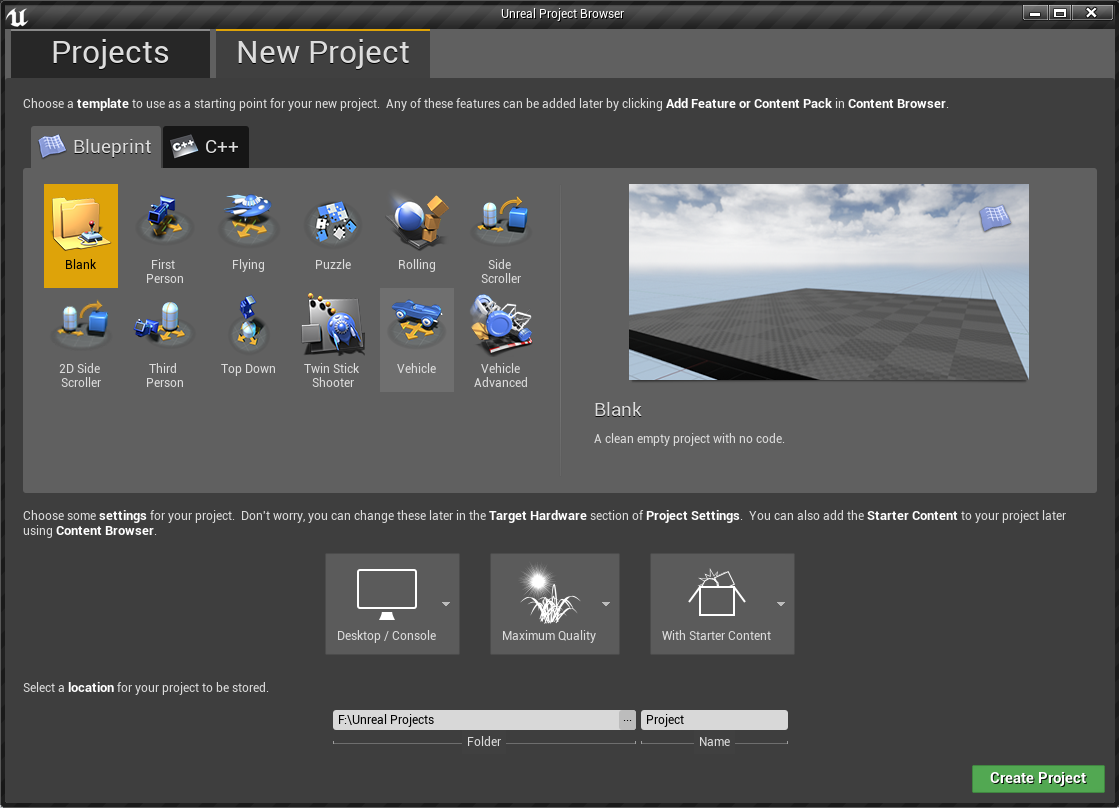
\includegraphics[scale=0.25]{Screeny/New_project}

Przeniesie nas to na ekran, na którym wybierzemy wstępne ustawienia naszego projektu. Pierwszą decyzją jaką musimy podjąć, to w jaki sposób będziemy rodzić sobie z logiką- poprzez pisanie kodu w C++, czy ustawianie bloków logicznych w tzw. Blueprint’ach.

Blueprint to system oparty na wizualny przesuwaniu bloków logicznych, zamiast ręcznego pisania kodu. System ten jest bardzo prostu w obsłudze. Każdy obiekt wymagający logiki może posiadac odpowiadający mu Blueprint. Pozwala to tworzenie skomplikowanej logiki bez konieczności pisania ogromnej ilości kodu. Blueprint, podobnie jak klasa w obiektowych językach programowania, może zostać użyty wielokrotnie. Na przykład stworzenie Blueprintu lampy, pozwoli ustawić ją w wielu miejscach w grze. Każda będzie działała tak samo.

Należy zaznaczyć, że wybór jednego sposobu, nie wyklucza nas całkowicie z korzystania z drugiej opcji. Jest to po prostu wskazanie, że preferujemy radzić sobie z logiką w taki, a nie inny sposób.
Warto również pamiętać, że Unreal Engine nie posiada dedykowanego edytora kodu C++. Jeśli chcemy programować w tym języku potrzebujemy zewnętrznego edytora, np. Visual Studio.

Kolejnym krokiem jest wybór schematu, jakim będziemy się posługiwać. W zależności od tego jaką grę tworzymy, scemat może zdecydowanie uprościć pierwsze kroki w edytorze gry (np. Schemat „2D Side Scroller”, stworzony z myślą o grach dwuwymiarowych, od razu będzie miał odpowiednio ustawioną kamerę). Istnieje również możliwość stworzenia pustego projektu, poprzez wybór opcji „Blank”.

Ostatnim krokiem jest wybór platformy na jaką chcemy tworzyć grę, jakość grafiki (istotna w przypadku słabszych sprzętów), oraz czy chcemy, by projekt zaimportował wstępne zasoby przygotowane dla nas przez Epic Games. Zasoby te składają sie między innymi z podstawowych animacji, tekstur i odgłosów.
Po dokonaniu wyboru pozostaje już tylko nazwac projekt i wcisnąć „Create Project”.

\section{Ekran główny}

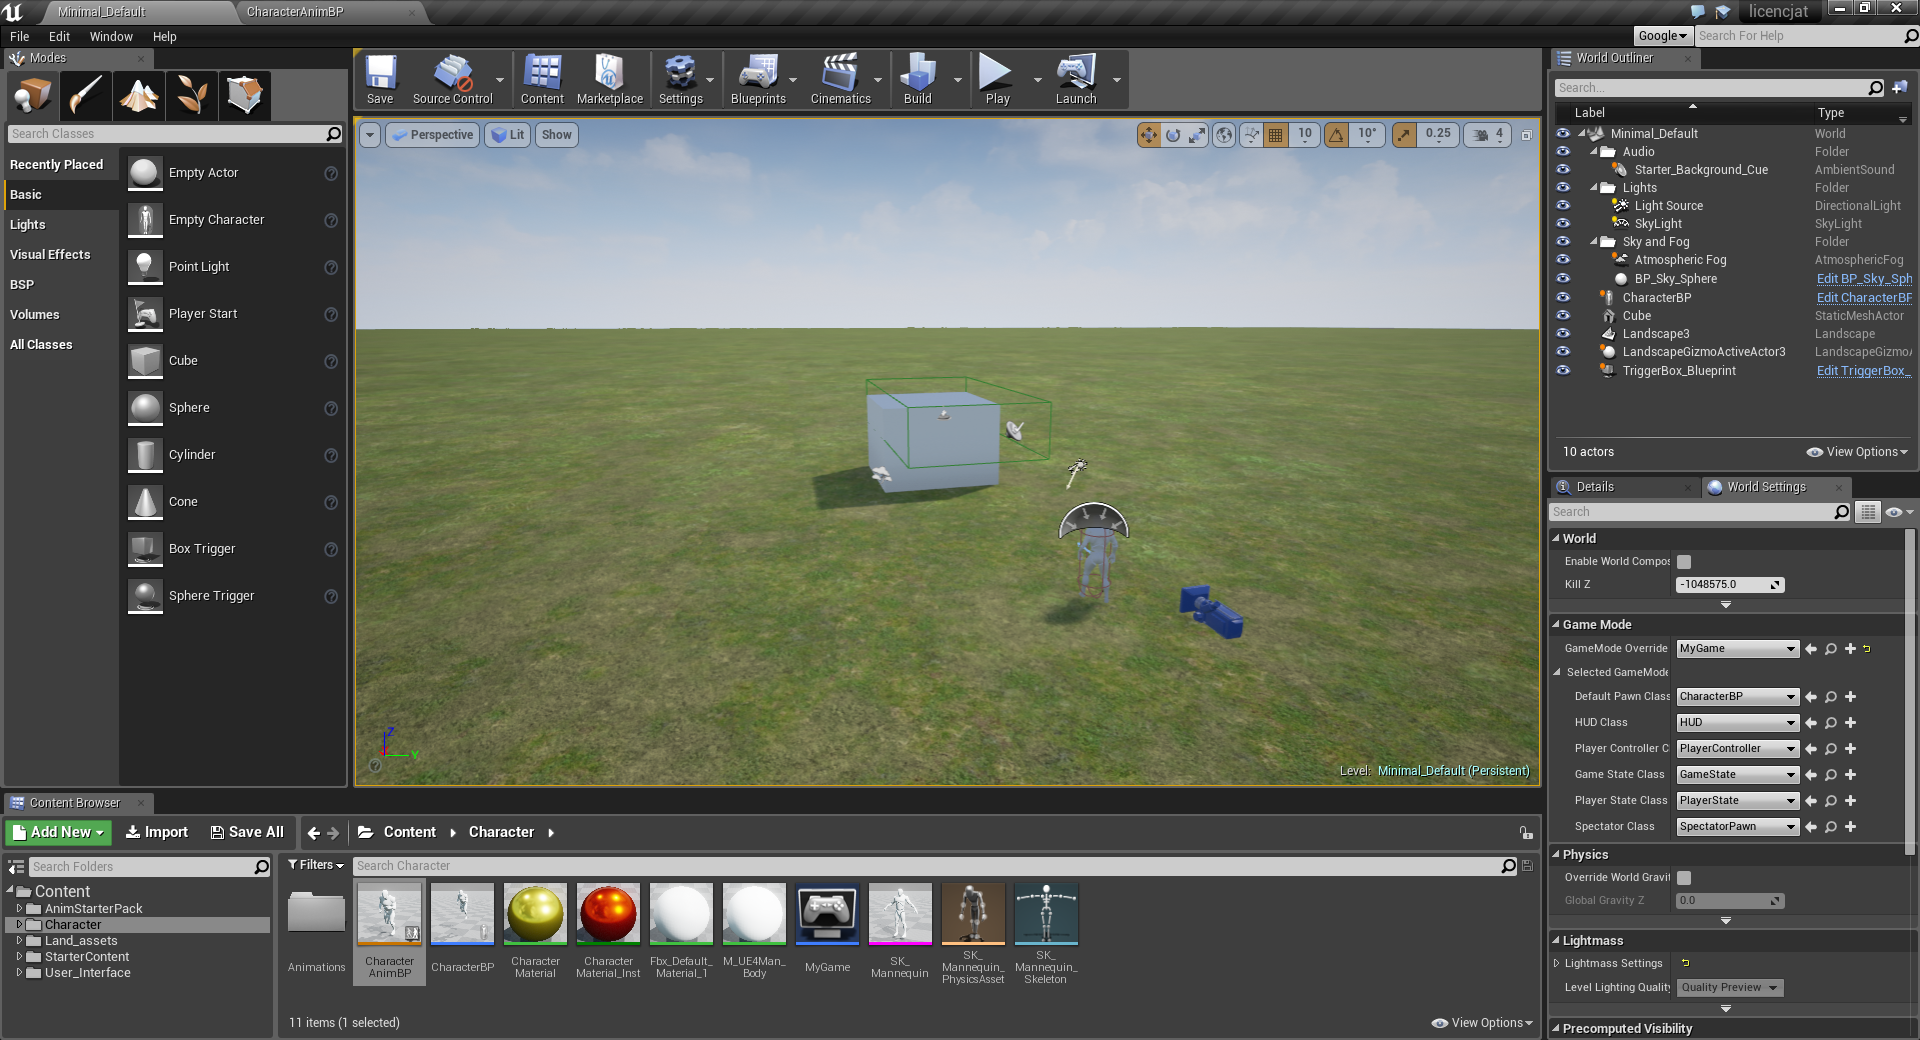
\includegraphics[scale=0.25]{Screeny/Main}

Po stworzeniu projektu, załaduje nam się ekran główny Unreal Engine. Na jego środku widzimy podgląd sceny nad którą obecnie pracujemy. Scena jest po prostu jednym z pozomów naszej gry.
Pod ekranem podglądu mamy przeglądarkę plików znajdujących się w projekcie. 

Po prawej stronie znajduje się lista obiektów, znajdujących się w obecnej scenie. Jako obiekt traktowane jest wszystko, od podłoża, przez postacie, aż po źródło światła, czy sam dźwięk.
Pod listą obiektów znajdują się szczegóły obecnie wybranego obiektu. 

Po lewej stronie znajdują się narzędzia do tworzenia obiektów. Jest to pięć zakładek zawierających w sobie wszystkie potrzebne opcje do tworzenia świata gry. Od tworzenia oświetlenia i prostych kształtów po nakładanie tekstur i modyfikowanie terenu.
 
\section{System Persona i Animacje}
Persona jest bardzo rozbudowanym narzędziem do edycji animacji. To jeden z najważniejszych systemów silnika. To dzięki niemu możemy okreslić gdzie, kiedy i w jakich warunkach  rozpoczyna się i kończy każda animacja w grze, od postaci, aż po spadające liście.

Trzeba pamiętać, że Unreal Engine nie posiada w sobie narzędzi do tworzenia animacji. Potrafi je tylko w pewnym stopniu modyfikować. Animacje należy importować z zewnętrznych programów do tworzenia animacji, takich jak Maya, lub Blender. Wystarczy przeciągnąć animację do przeglądarki plików.

Aby uruchomić Personę, wystarczy dwa razy kliknąć w edytorze na dowolny obiekt związany z animacją (np. Sama animacja, lub Blueprint animacji).

Sam system składa się z czterech głównych trybów, ukazanych w prawym górnym rogu okienka.

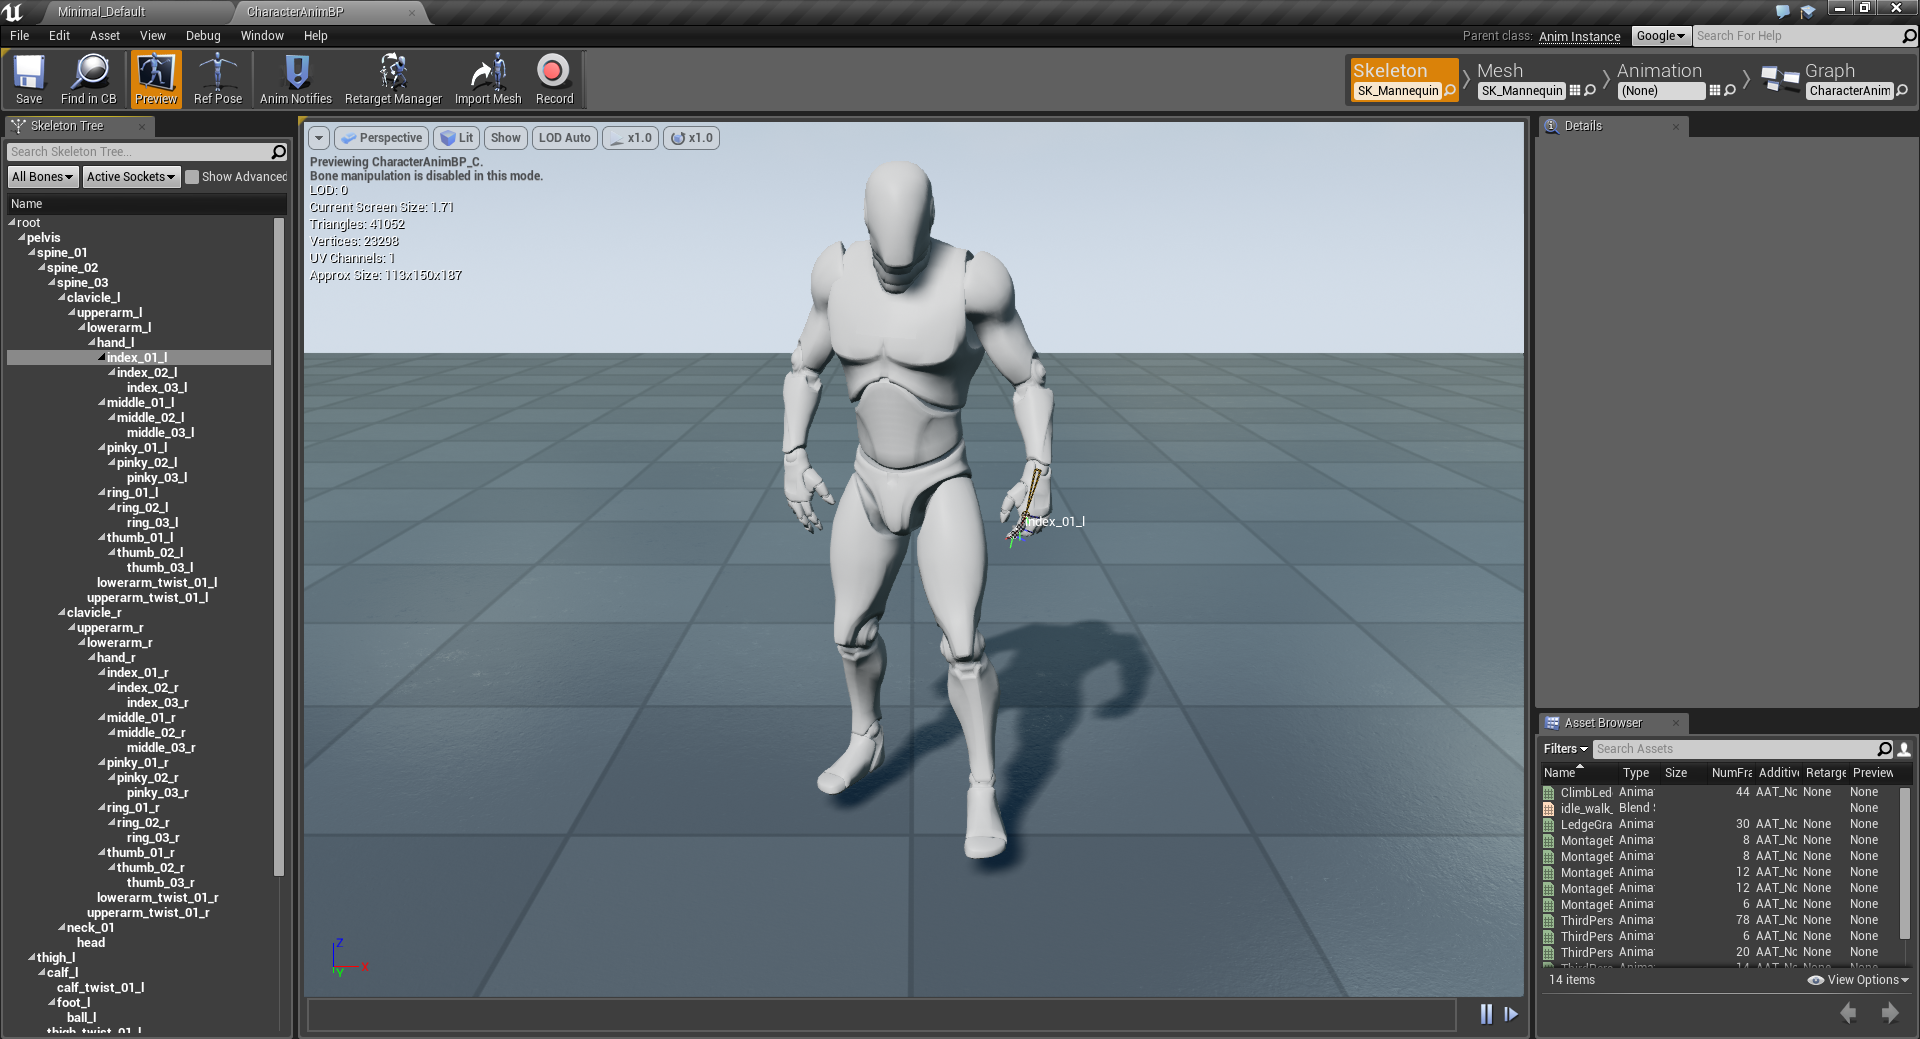
\includegraphics[scale=0.25]{Screeny/Skeleton}

Pierwszy tryb odpowiada za edycję szkieletu animacji. Po uruchomieniu od razu rzuca się w oczy podgląd animacji na środku okna. Rejestruje on obecny stan animacji. Podgląd ten jest częścią wspólną wszystkich trybó pracy w Personie.
Po lewej stronie wyświetlone są wszystkie wnęki i połączone z nimi kości obecnego modelu. Można dowolnie dodawać je i usuwać ze szkieletu postaci. Jest to szczególnie przydatne, gdy chcemy aby nasza postać np. chwytała broń. Wystarczy dodać wnękę do ręki szkieletu i już jest to możliwe.

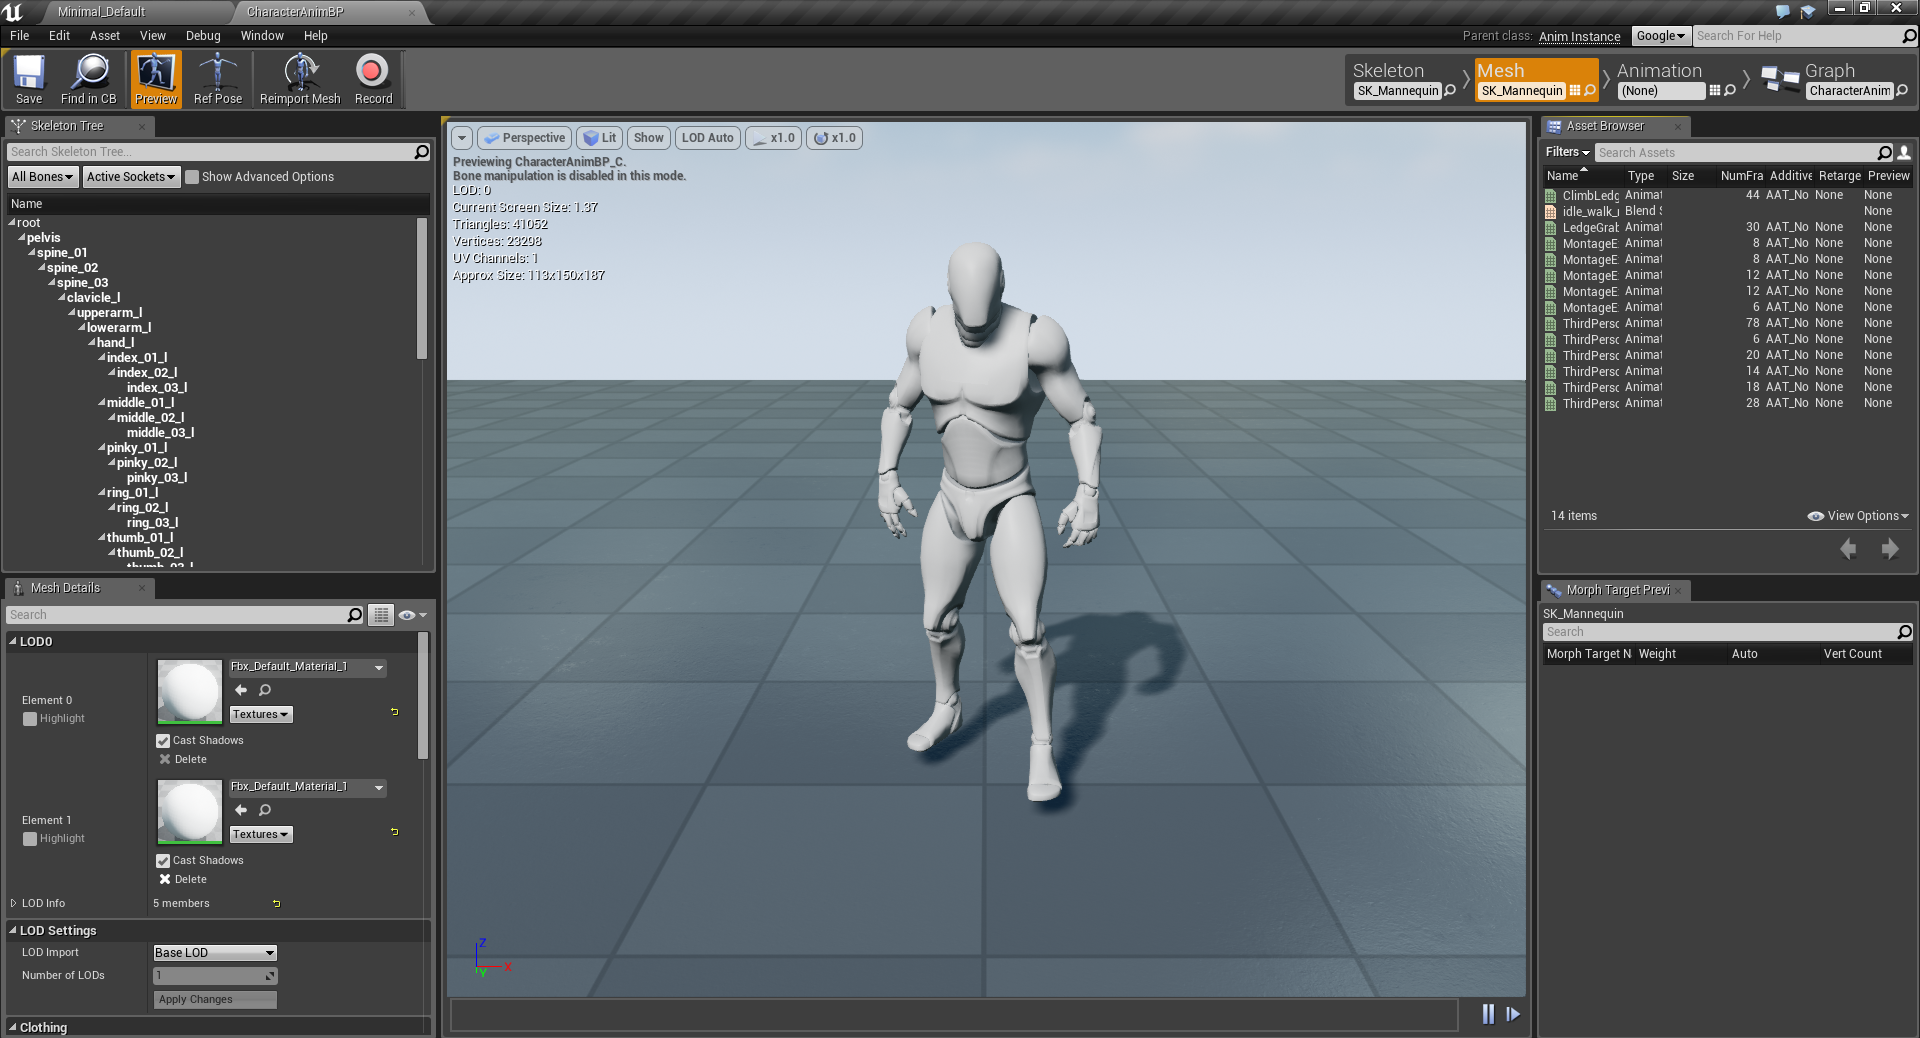
\includegraphics[scale=0.25]{Screeny/Mesh}

Kolejny ekran jest odpowiedzialny za edycję meshy. Mesh to nic innego ja zbiór punktów, linii i wieloboków, które składają się na ostateczny kształt obiektu.
Ten tryb ma wiele wspólnego z poprzednim. Ma jednak dwa ważne menu, niedostępne w innych podsystemach Persony – „Mesh Details” i „Morph Target Preview”.
Mesh Details odpowiada głównie za edycję mesh’u nad którym obecnie pracujemy. Możemy dodać do niego nowe tekstury, kontrolować właściwości fizyczne (np. Płaszcz łopoczący na wietrze), lub umożliwić kolizję z innymi obiektami w grze.
Morph Target Preview pozwala na podgląd wszystkich modyfikacji mesha. Możemy na przykład zmienić wyraz twarzy postaci, zapisać go i użyć w odpowiedniej sytuacji, a potem obejżeć go bez konieczności trwałej zmiany samego mesha.

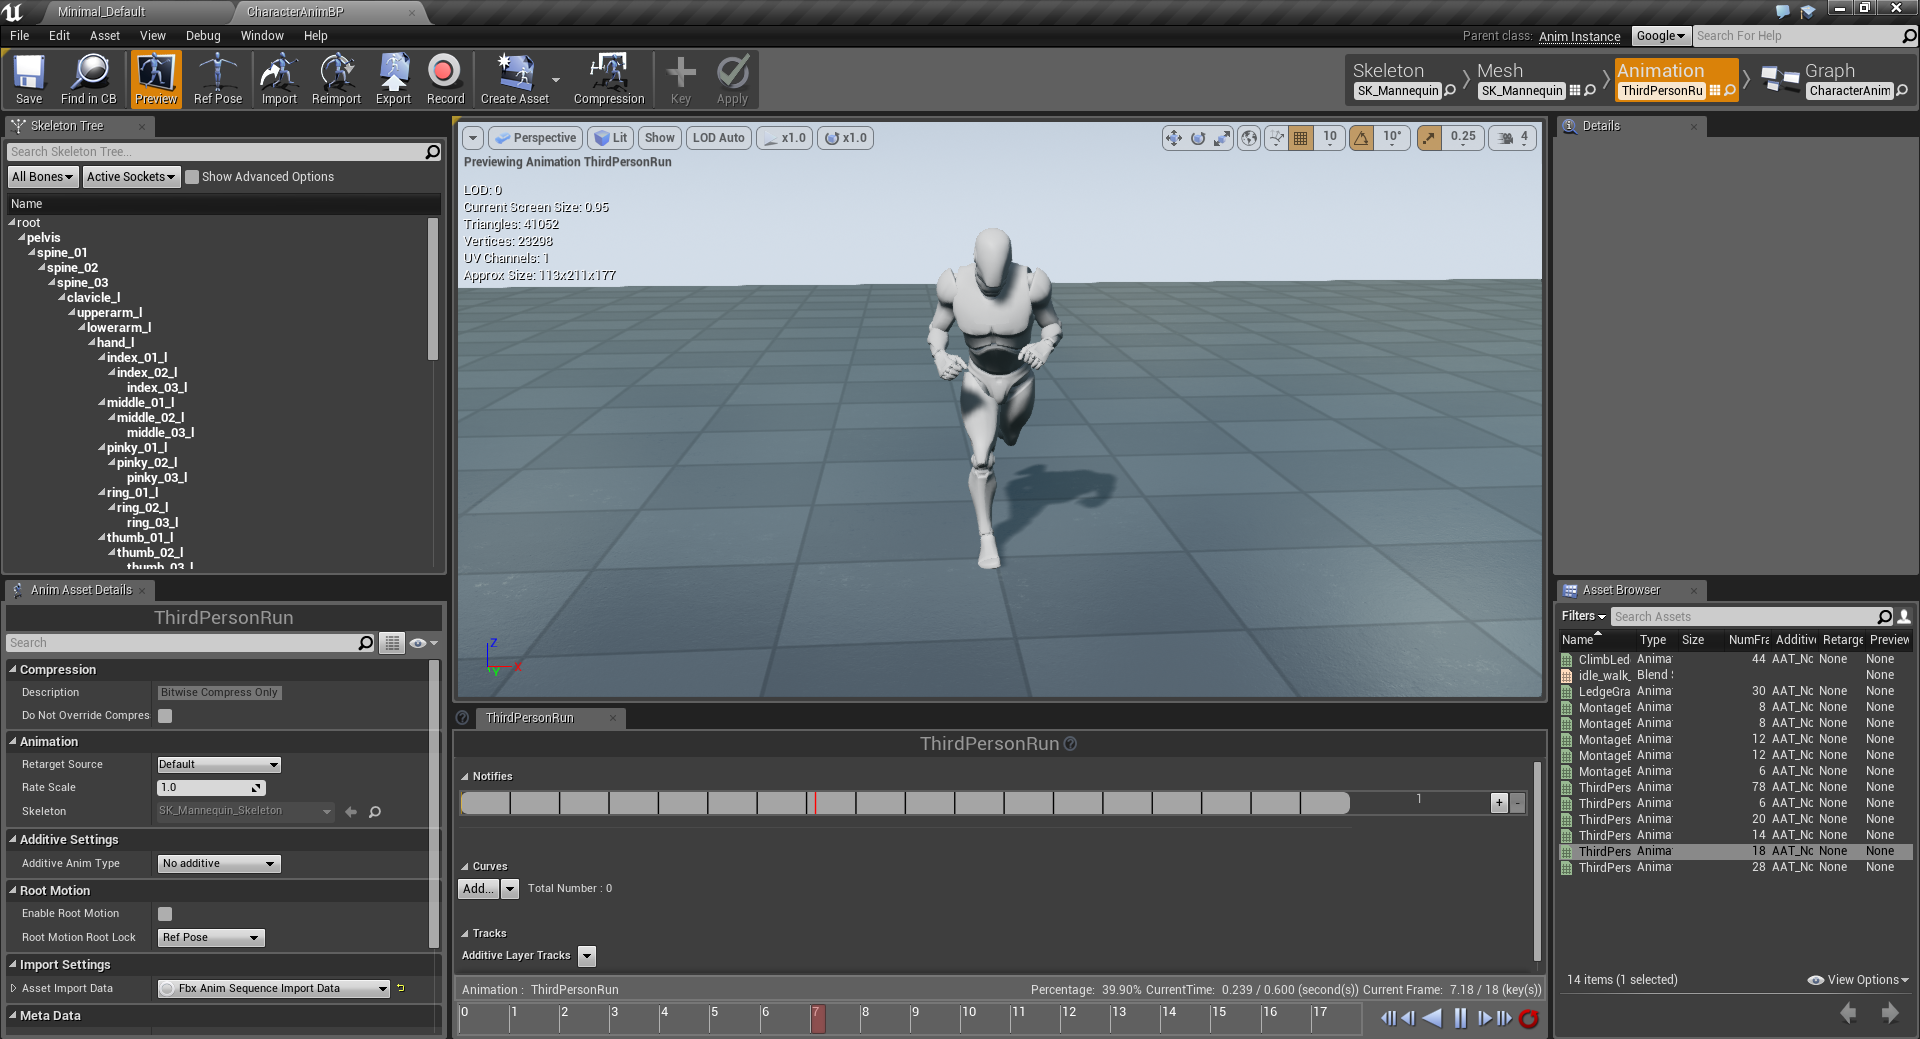
\includegraphics[scale=0.25]{Screeny/Animation}

Następny tryb daje nam kontrolę nad animacjami. W lewym dolnym rogu widzimy szczegułowe ustawienia wybranej w tym momencie animacji.
Pod oknem podglądu animacji widzimy narzędzie dzięki któremu możemy przewijać wybraną animację klatka po klatce. Po wybraniu interesującego nas momentu animacji, możemy dodać różnego rodzaju efekty np. w momencie, gdy model w animacji biegu dotyka ziemi, możemy dodać odgłos kroku, albo efekt, który wznieci tuman kurzu pod stopą modelu.

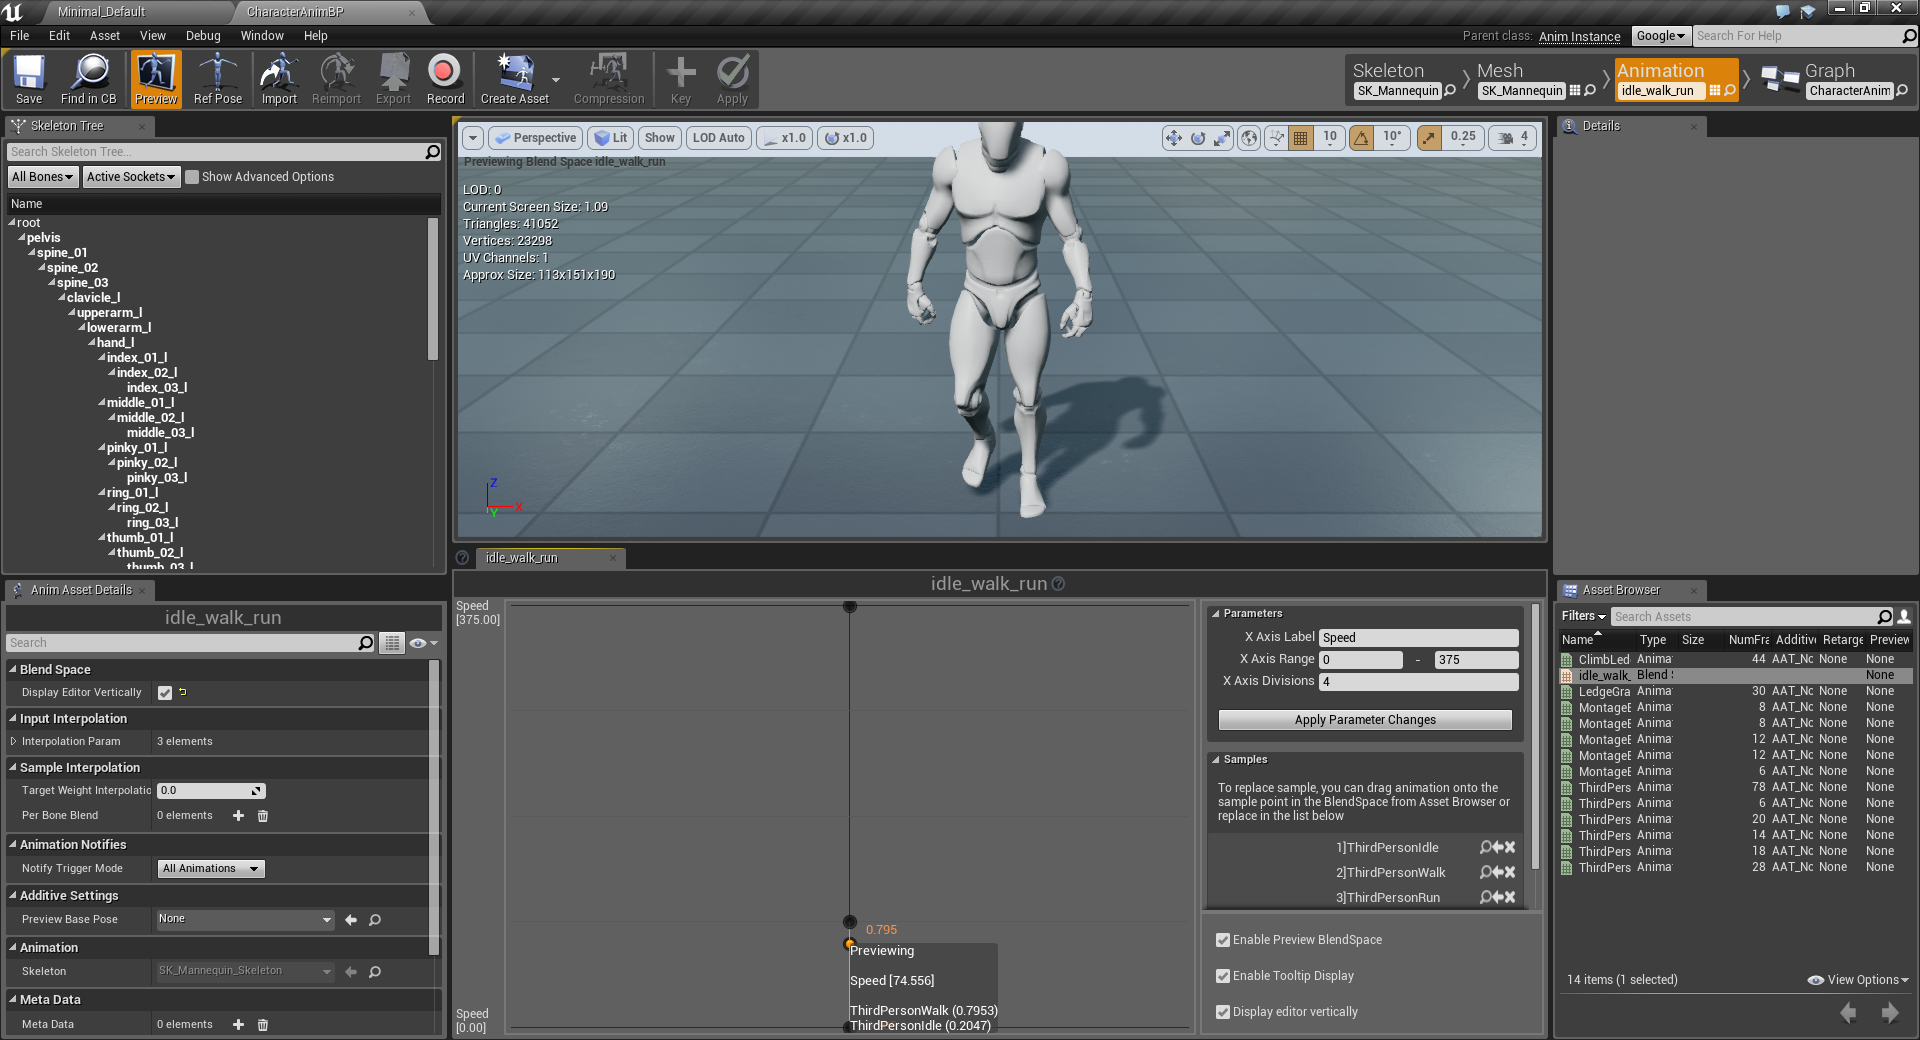
\includegraphics[scale=0.25]{Screeny/Blend_Space}

Warto również wspomnieć o tzw. „Blend Spaces”, czyli możliwość łączenia kilku animacji w jedną. Tej metody używa się, gdy zajdą ustalone okoliczności. Gwarantuje to płynność w przechodzeniu między animacjami. Na przykład, stojąca postać pod wpływem wciśnięcia przycisku zaczyna iść (wartość zmiennej „prędkość” zwiększa się). Jeśli gracz nie puści przycisku, chód zamienia się w bieg.
Aby stworzyć Blend Space, wystarczy kliknąć prawym przyciskiem myszy w przeglądarce plików, w ekranie głównym. Potem z menu kontekstowego wybieramy Animation > Blend Speaces

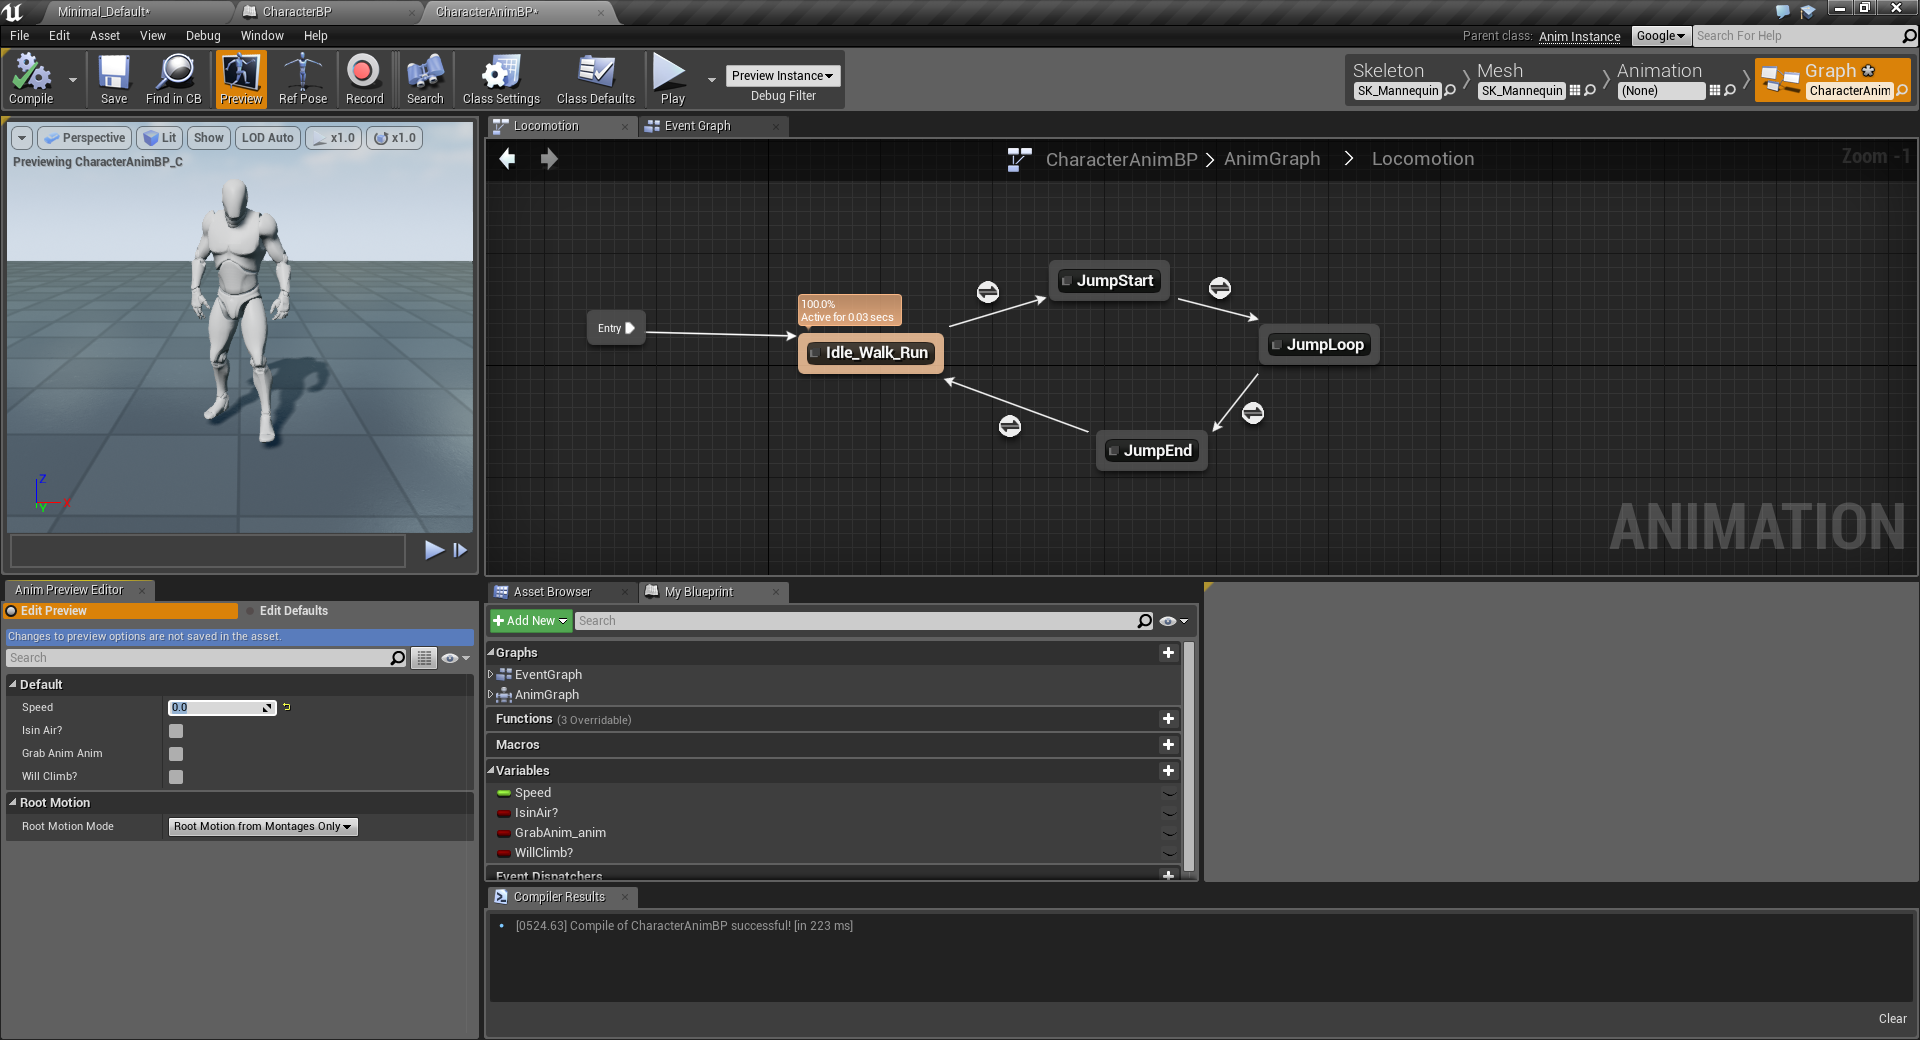
\includegraphics[scale=0.25]{Screeny/AnimGraph_Event}

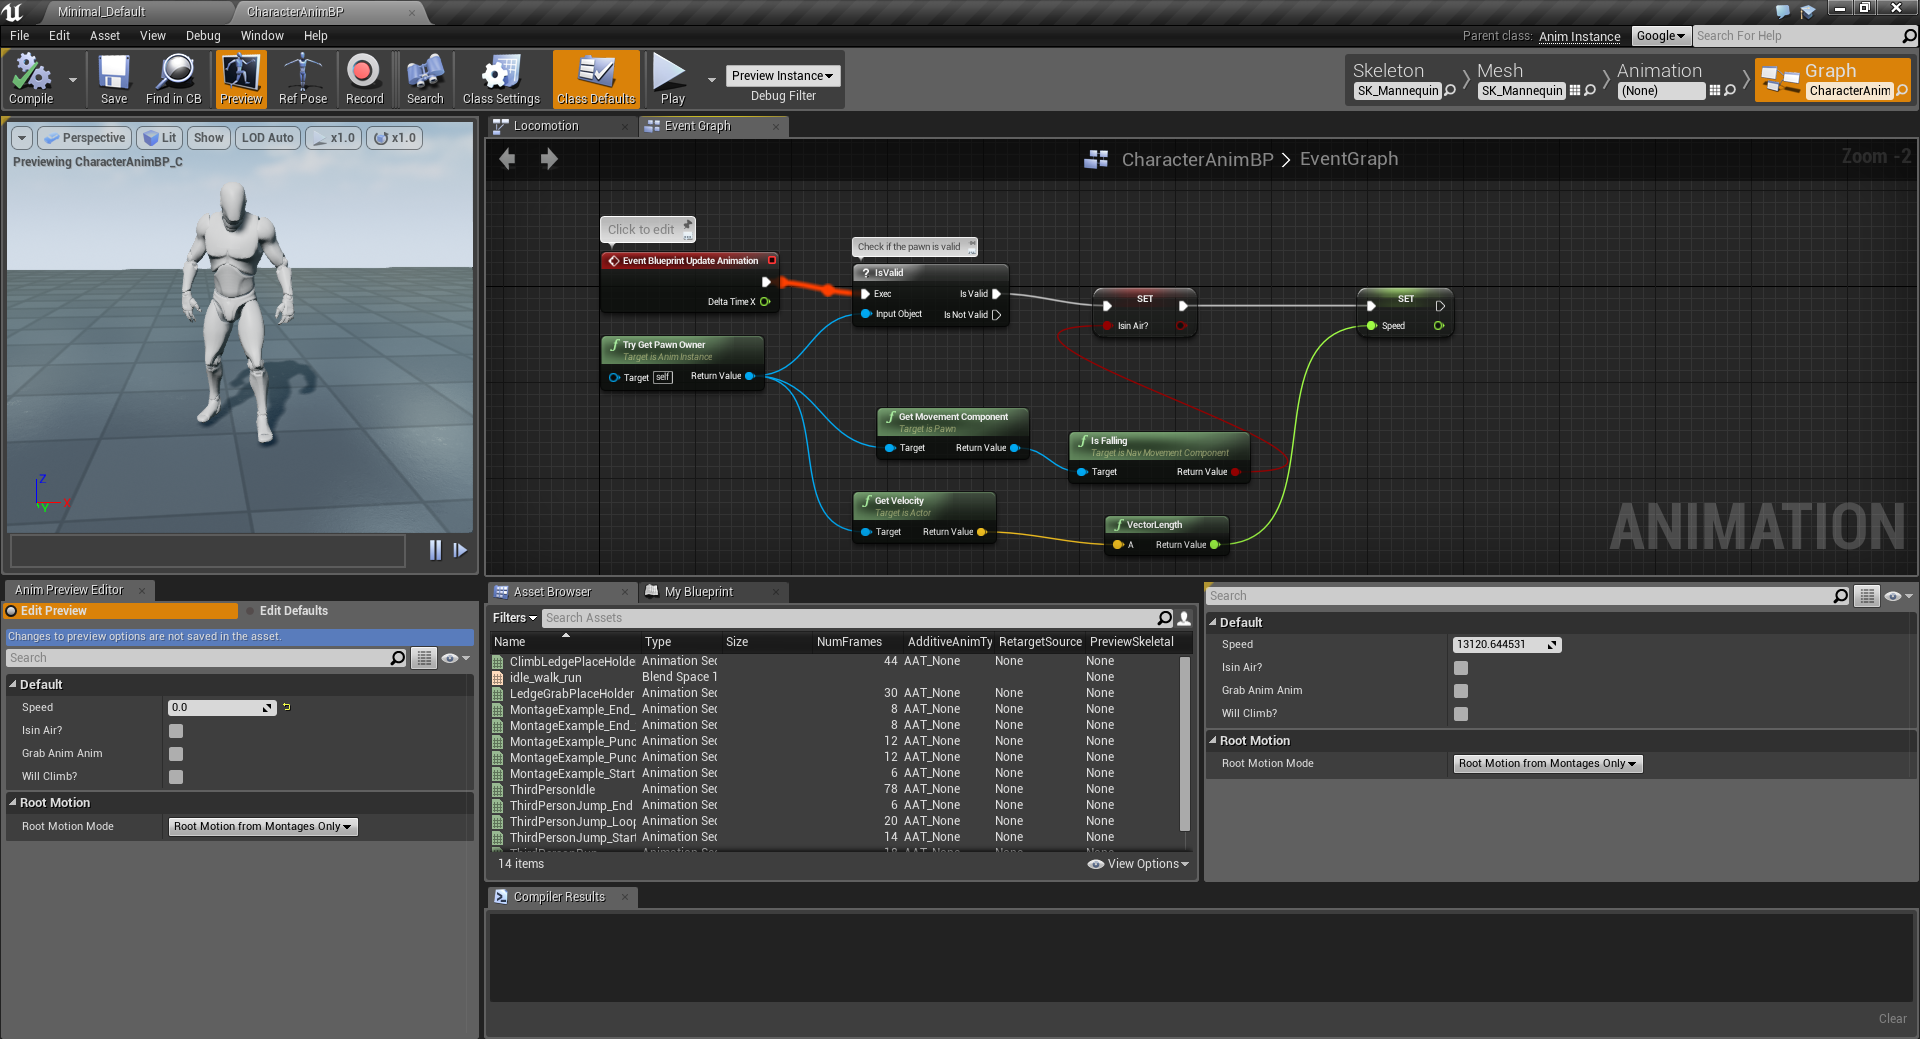
\includegraphics[scale=0.25]{Screeny/EventGraph_Event}

Ostatnią opcją Persony jest ekran grafów. Dzieli się on na dwa ekrany- Graf animacji, oraz graf zdarzeń. Każdy Blueprint związany z animacją posiada oba grafy.
Graf zdarzeń określa wszystkie zdarzenia jakie muszą zajść, aby odtworzona została konkretna animacja w grze. Najczęściej robi się to poprzez modyfikowanie zmiennych zadeklarowanych w grafie. Zmiany zachodzą pod konkretnymi warunkami w grze.

Graf animacji korzysta z grafu zdarzeń, by określić finalną pozę mesh’u w danej klatce. Używa on głównie logiki zawartej w grafie zdarzeń, aby określić czy powinny zajść zmiany. Na przykład, gdy gracz wciska przycisk skoku, wcześniej przygotowany graf zdarzeń może zarejestrować, że powinno to zmienić wartośc bolleanu „skok” na True.  Graf animacji rejestruje zmianę i zmienia animację z biegu na skok.

W następnym rozdziale przyjżymy się bliżej tym systemom i zaprezentujemy je w praktyce.

\chapter{ Testowanie gier}

Wśród programistów gier panuje przekonanie, że tworzenie zautomatyzowanych testów do gier jest pozbawione sensu. Większość firm zatrudnia sztab testerów, którzy manualnie sprawdzają najdrobniejsze elementy danej gry. Wynika to z kilku wyjątkowych cech tworzenia gier.

Po pierwsze, zdecydowana większość logiki używanej w grach zależy od czynników, które nie są do końca deterministyczne. Oznacza to, że warunki w jakich użytkowana będzie gra często mogą być przypadkowe i niemożliwe do przewidzenia. Na przykład, gra może być uruchamiana na setkach różnych konfiguracji sprzętu. Przetestowanie każdej z nich jest niemożliwe. Dodajmy do tego fakt, że sprzęt może znajdować się w gorącym pomieszczeniu, co pogorszy jego osiągi. W tle mogą również być uruchomione inne programy, które zajmują zasoby danego sprzętu. To tylko kilka przykładów czynników nad którymi twórcy gier nie mają żadnej kontroli. Ustalenie standardu według którego możnaby napisac test, w takich warunkach jest niemal niewykonalne.

Innym problemem jest, że większość wyników produkowanych przez grę jest niemożliwa do zmierzenia. 
W grach generowane są takie elementy jak grafika i dźwięk.  Skuteczność efektów wizualnych, jak i dźwiękowych jest rzeczą załkowicie subiektywną. Nie da się określić automatycznym testem czy muzyka jest dostatecznie głośna, lub czy dana tekstura wygląda dobrze w danym miejscu. Wszystko zależy od wizji twórcór gry. W takim wypadku jedyny możliwy test, to test manualny.

Kolejną przeszkodą jest fakt, że w większości gier wszystkie mechaniki i podsystemy składają się na jedną spójną całością. W grach stworzonych na potrzeby tego projektu zaimplementowaliśmy mechanikę wspinaczki. Aby działała, zarówno fizyka gry, jak i animacje oraz kod wykrywający kolizję muszą działać poprawnie. W przypadku porażki nie sposób na pierwszy rzut oka okreslić, który z tych systemów zawiódł. Możemy napisać testy, które sprawdzą wszystkie po kolei, jednak wszelkie wyniki jakie dostaniemy będą wyrwane z kontekstu i nie powiedzą co się stało, gdy wszystkie czynniki złączyły się w jedną całość. W związku z tym tu również musimy zdać się na testowanie ręczne.

Mimo powyższych problemów, pisanie unit testów do gier nie jest całkowicie niemożliwe. Wymaga to jednak bardzo specyficznych warunków. Głównym warunkiem jest określenie testów jeszcze przed rozpoczeciem programowania samej gry. Jest to jednak niepraktyczne podejście, które wiąże ręce twórcom gry.

Gry stworzone na potrzeby projektu zostały przetestowane wyłącznie manualnie. Testowaliśmy głównie mechanikę skoku, wspinaczki i biegu, ponieważ są to główne elementy naszych gier.



\chapter{Podsumowanie procesu tworzenia gier dla obu silników}

cos


% zakończenie
\summary
Możliwości, jakie stoją przed archiwum prac magisterskich opartych na
XML-u, są ograniczone jedynie czasem, jaki należy poświęcić na pełną
implementację systemu. Nie ma przeszkód technologicznych do stworzenia
co najmniej równie doskonałego repozytorium, jak ma to miejsce w
przypadku ETD. Jeżeli chcemy w pełni uczestniczyć w rozwoju nowej ery
informacji, musimy szczególną uwagę przykładać do odpowiedniej
klasyfikacji i archiwizacji danych. Sądzę, że język XML znacznie to
upraszcza.

% załączniki (opcjonalnie):
\appendix
\chapter{Tytuł załącznika jeden}

Treść załącznika jeden.

\chapter{Tytuł załącznika dwa}

Treść załącznika dwa.

% literatura (obowiązkowo):
\bibliographystyle{unsrt}
\bibliography{xml}

% spis tabel (jeżeli jest potrzebny):
\listoftables

% spis rysunków (jeżeli jest potrzebny):
\listoffigures

\oswiadczenie

\end{document}
